\chapter{Einleitung}

Ziel eines Teilchenbeschleuniger ist es einen Teilchenstrahl oder -bunch zu beschleunigen und m�glichst 
fokussiert auf einer Sollbahn zu halten. Einerseits um keine Teilchen zu verlieren, anderseits um z.B.
bei einem Collider die Teilchendichte hoch zu halten.
In unserem Versuch werden wir mit einem einfachen Linearbeschleuniger arbeiten und die Energie sowie die Emittanz,
eine die Qualit�t des Strahls charakterisierende Gr��e, die wir im Theorieteil erkl�ren werden, zu messen.

\section{Aufbau}
\begin{figure}[ht]
  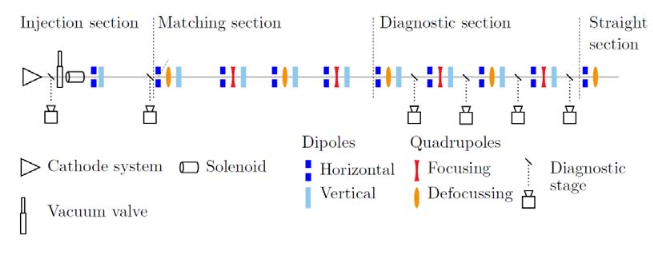
\includegraphics[width=0.8\textwidth]{./salome-aufbau.png}
  \caption{( Matching section wurde abgebaut)}
\end{figure}

Der Teilchenbeschleuniger besteht aus einem Kathodenstrahler zur Erzeugung des Strahls, einer Spule 
(Solenoidmagnet) dessen �u�ere Streufelder fokussierend wirken, einigen Dipol- und Quadromagneten.

\begin{figure}[]
  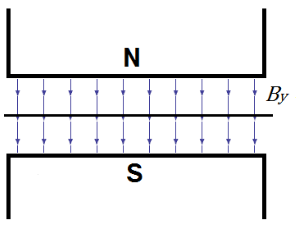
\includegraphics[width=0.40\textwidth]{./dipol.png}\hfill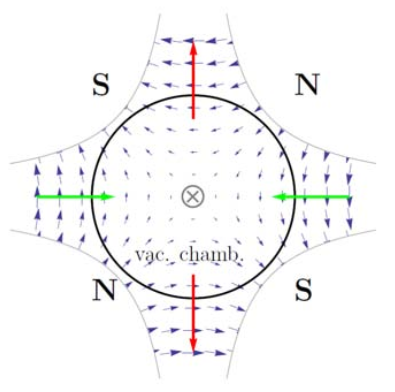
\includegraphics[width=0.40\textwidth]{./quadropol.png}
  \caption{Di-und Quadropolschemata} \label{fig:magnete}
  
\end{figure}
\newpage
Wie man im Bild \ref{fig:magnete} illustriert sehen kann erzeugt der Dipolmagnet ein homogenes Magnetfeld in (vertikale) y-Richtung,
das daf�r geeignet ist externe Magnetfelder wie das Erdmagnetfeld zu kompensieren. 
Nehmen wir ein idealisierten Teilchenstrahl an, so lenkt  der Dipol den Strahl auf 
eine Kreisbahn $\frac{e}{p} B_y(x)=\frac{1}{R}$.

P:Impuls in Richtung der Sollbahn

R:Raidus der Kreisbahn

Die St�rke des Dipols werden wir im Folgendem damit charakterisieren.
Der Quadropol h�ngt linear von x ab und wirkt in einer Ebene fokussierend in der Anderen defokussierend, 
deswegen werden sie um 90� gedreht hintereinander aufgebaut.

$\frac{e}{p} B_y(x)=kx$

$\frac{e}{p} B_x(y)=-ky$

$k$: St�rke des Quadrupolmagneten

\newpage
\section{Theorie}
\section {Phasenraum, Emittanz und Twissparameter}
Man stellt zun�chst die Bewegungsgleichungen eines einzelnen Teilchens auf und guckt wie dieses sich unabh�ngig 
von den anderen Teilchen im Bezug auf die Sollbahn bewegt. Den Einfluss der Teilchen aufeinander kann hier 
vernachl�ssigt werden da der Strom sehr klein ist und vorrausgesetzt wird, dassdie Sollbahn nicht gekr�mmt ist.

\begin{equation}x''(s)-k(s)x(s)=0
\end{equation}

\begin{equation}y''(s)+k(s)y(s)=0
\end{equation}

s parametrisiert die Sollbahn.

Die Herleitung der Differentialgleichung findet man im Wille Kapitel ``Linear beam optics''.  

Hier sieht man das die Bewegung in x und y Richtung entkoppelt ist und die

Fokussierung/Defokussierung in beiden Ebenen gerade umgekehrt ist.

Die L�sung der Gleichung ist analytisch schwierig, da sich k entlang der Bahn s �ndert, jedoch kann man jeden Abschnitt in der Sollbahn wo sich
k �ndert f�r sich betrachten und so ein Kalk�l entwickeln der die Bewegungsgleichung in diskreten Abschnitten mithilfe von Matrizen l�st.
M�chte man zb. f�r gegebene Anfangswerte x0 und x'0 des Teilchens die Werte x1, x'1 ermitteln nachdem es einen Dipol und Quadropol durchlaufen hat,
so nimmt man die einzelnen Matrizen f�r Dipol und Quadropol und f�hrt sie hintereinander aus.

Diesen Kalk�l werden wir sp�ter in der Berechnung der Emittanz verwenden.

Das Teilchen f�hrt eine oszillierende Bewegung um die Sollbahn durch.Im Phasenraum ist die Bewegung durch eine Ellipse beschrieben:

\begin{equation}
\epsilon=\gamma(s)x^2(s)+2\alpha(s)x(s)x'(s)+\beta(s)x'^2(s)\end{equation}

x(s) ist die Ablenkung zur Sollbahn, x'(s) Der Winkel zwischen Geschwindigkeit und Sollbahn. 

$\gamma(s),\alpha(s),\beta(s)$ sind die sogenannten ``Twissparameter'', sie bestimmen die Form und Position der Ellipse, und sind
auch abh�ngig von der Position auf der Sollbahn. Sie werden allein durch den Aufbau bzw. der Fokussierung entlang der Sollbahn 
bestimmt und unabh�ngig von den Anfangsbedingungen.

Die Anfangsbedingungen x0 und x'0 gehen in die Integrationskonstanten $\epsilon$ und der Anfangsphase $\Phi$ der Schwingung ein.

$\epsilon$ ist die sogenannte Emittanz des Teilchens und wurde als Integrationskonstante eingef�hrt. Sie ist daher eine 
Erhaltungsgr��e und nach der Gleichung im Phasenraum auch die Fl�che der Ellipse bis auf einen Faktor $\pi$.
Sie charakterisiert somit die Qualit�t und die Fokussierbarkeit des Strahls.

Im n�chsten Schritt wollen wir charakteristische Gr��en f�r den Teilchenstrahl, bestehend aus mehreren Teilchen die den selben Differentialgleichungen
unterliegen, festlegen. Da die Twissparameter unabh�ngig von den Anfangsbedingungen die Ellipse entlang s verformen, liegen Teilchen mit gleicher Emittanz
an verschiedenen Punkten derselben Ellipse oder sie haben verschiedene Emittanzen und bewegen sich innerhalb einer kleineren bzw. gr��eren Ellipse.

Wir definieren die Emittanz des gesamten Teilchensstrahles als die Fl�che der Ellipse die von der Standardabweichungen von x und x' aufgespannt wird.

Da sich die so definierte Emittanz mit Beschleunigung verkleinert f�hren wir die normierte Emittanz ein :

\begin{equation}
\epsilon_n=\gamma \beta \sqrt{<x^2>*<x'^2>-(<xx'>)^2}\end{equation}

mit dem Lorentzfaktor $\gamma$ und $\beta=v/c$